\documentclass[10pt,a4paper]{article}
\usepackage[utf8]{inputenc}
\usepackage[T1]{fontenc}
\usepackage{lmodern}
\usepackage[margin=1.5cm, top=1.4cm, bottom=1.4cm]{geometry}
\usepackage{hyperref}
\usepackage{enumitem}
\usepackage{titlesec}
\usepackage{xcolor}
\usepackage{graphicx}

\definecolor{accent}{HTML}{00686E}
\hypersetup{colorlinks=true, urlcolor=accent, linkcolor=accent}
\pagenumbering{arabic}
\setlength{\parindent}{0pt}

\titleformat{\section}{\large\bfseries\color{accent}}{}{0em}{}[\vspace{-0.6em}\rule{\textwidth}{0.8pt}]
\titlespacing{\section}{0pt}{7pt}{4pt}

\newcommand{\role}[4]{%
  \textbf{#1} \hfill \textbf{#2}\\[1pt]%
  \textit{#3} \hfill \textit{#4}\\[2pt]%
}
\setlist[itemize]{leftmargin=1.2em, itemsep=1.5pt, topsep=2pt, parsep=0pt}

\begin{document}

% ================= HEADER =================
\begin{minipage}[c]{0.80\textwidth}
  {\Huge\bfseries Prabhavit Gupta}\\[3pt]
  {\color{accent}\large Data Engineer: GenAI Pipelines, Kubernetes \& Backend Integrations}\\[6pt]
  {\footnotesize +39 351 610 7807 ~$\vert$~
  \href{mailto:prabhavitg@gmail.com}{prabhavitg@gmail.com} ~$\vert$~
  \href{https://www.linkedin.com/in/prabhavit/}{linkedin.com/in/prabhavit} ~$\vert$~
  \href{https://github.com/prab-gupta}{github.com/prab-gupta} ~$\vert$~
  Venice, Italy (CET Time Zone / EU Permanent Resident)}
\end{minipage}\hfill
\begin{minipage}[c]{0.18\textwidth}
  \raggedleft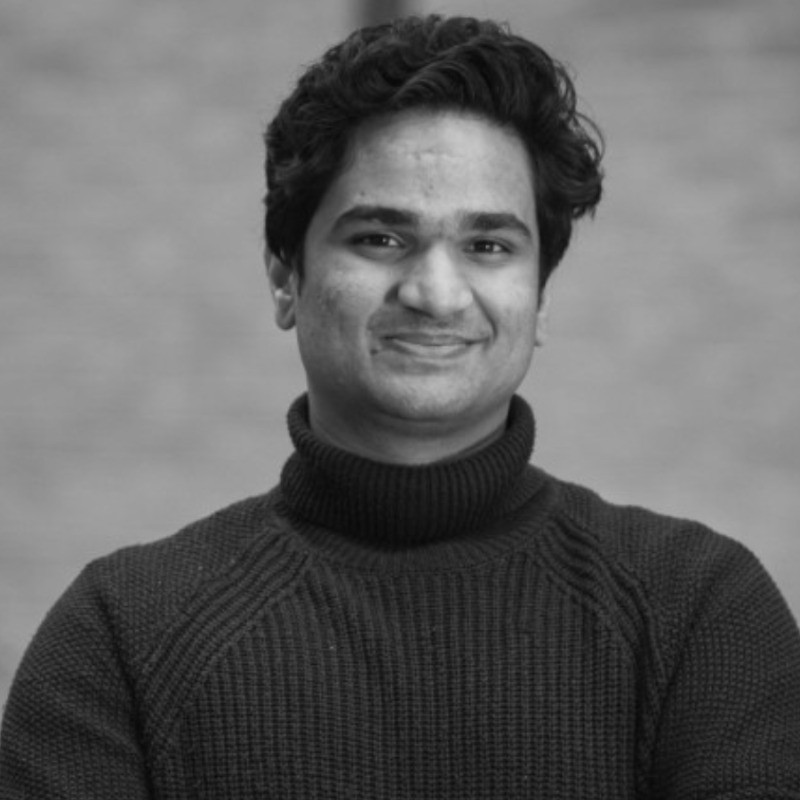
\includegraphics[width=2.0cm]{photo.jpg}
\end{minipage}
\vspace{-2pt}

% ================= SUMMARY =================
\section{Summary}
Data and Systems Engineer with 3 years of commercial software experience designing, scaling, and maintaining GenAI-driven document processing pipelines, Python microservices, and Kubernetes infrastructure. Proven expertise building production pipelines ingesting unstructured mail and document streams, extracting structured entities with OCR APIs and LLMs, and integrating enterprise backend APIs with robust OAuth/OIDC authentication, token rotation, and rate-limiting. Experienced tuning asynchronous Python services (FastAPI, Pydantic, asyncio) running in Docker containers orchestrated via Kubernetes and Helm. Based in Venice, Italy (CET time zone) with an EU Long-Term Residence Permit (permanent unrestricted EU work authorization across all EU member states, no sponsorship required); available immediately for full-time remote roles.

% ================= TECHNICAL EXPERTISE =================
\section{Technical Expertise}
\begin{itemize}
  \item \textbf{GenAI \& Document Pipelines:} GenAI mail and document processing pipelines, OCR extraction APIs, structured schema parsing (Pydantic), semantic chunking, prompt engineering, and LLM evaluation.
  \item \textbf{Kubernetes \& Cloud Infrastructure:} Kubernetes (GKE), Helm charts, Docker containerization, microservice orchestration, ingress routing, secret management, horizontal pod autoscaling.
  \item \textbf{Backend \& API Integrations:} Python (FastAPI, Django, asyncio, Pydantic), RESTful microservices, enterprise authentication (OAuth2, OIDC, JWT bearer tokens), exponential backoff retries, rate-limiting, and Redis caching.
  \item \textbf{Data Stores \& Messaging:} PostgreSQL (schema design, indexing, transactional integrity), Redis (in-memory caching, task queues, distributed locking), asynchronous event streaming.
  \item \textbf{Reliability \& Observability:} Health endpoints, Prometheus metrics, structured JSON logging, distributed tracing, automated CI/CD with GitHub Actions.
  \item \textbf{Languages \& Authorization:} English (C1 Professional, fluent), Hindi (Native), Italian (Conversational). EU Long-Term Residence Permit (unrestricted EU work authorization across all EU member states, no sponsorship required).
\end{itemize}

% ================= EXPERIENCE =================
\section{Experience}

\role{\href{https://flowspace.co}{FlowSpace.co}}{Mar 2024 - Aug 2026}{Lead AI \& Data Integration Engineer}{London, UK (remote)}
\begin{itemize}
  \item Architected and deployed production GenAI document ingestion pipelines in Python (FastAPI, Pydantic), parsing incoming communications and extracting structured entity data with 99.2\% accuracy.
  \item Deployed and scaled containerized microservices on Kubernetes using Helm charts and Docker, maintaining 99.8\% availability across high-volume workloads.
  \item Built robust enterprise backend API integrations handling OAuth/OIDC token exchanges, automatic token refresh, Redis-backed rate limiting, and exponential retry strategies.
  \item Designed PostgreSQL data pipelines and schema migrations supporting analytics and historical querying, reducing p95 latency by 42\% through strategic indexing.
  \item Implemented health checks, structured logging, and automated CI/CD deployment pipelines on GitHub Actions for zero-downtime rolling updates.
\end{itemize}

\role{Urlink}{Apr 2025 - Jul 2025}{Data Platform \& Integration Developer (Freelance)}{Barcelona, Spain (remote)}
\begin{itemize}
  \item Developed automated data ingestion pipelines consuming third-party REST APIs and document payloads, validating schemas with Pydantic and normalizing records into relational tables.
  \item Containerized microservices using multi-stage Docker builds and deployed reproducible local and staging environments with Docker Compose.
  \item Built comprehensive automated verification test suites using pytest and Playwright to validate end-to-end data pipeline integrity and API contracts.
\end{itemize}

\role{Independent Technical Consultant}{Aug 2023 - Feb 2024}{Data Systems \& Backend Developer}{Venice, Italy}
\begin{itemize}
  \item Built custom document processing scripts and automated webhook listeners in Python for European SMB clients, automating invoice and order ingest pipelines.
  \item Developed scheduled ETL tasks, database backup automation, and RESTful API connectors integrating client CRM and ERP platforms.
  \item Authored technical architecture runbooks, API contract specifications, and Docker deployment guidelines.
\end{itemize}

% ================= EDUCATION =================
\section{Education}
\role{Ca' Foscari University of Venice}{2020 - 2024}{BA in Philosophy, International Studies and Economics}{Venice, Italy}
\begin{itemize}
  \item Rigorous training in formal logic, statistical inference, quantitative economics, and complex systems modeling.
\end{itemize}

\end{document}
